\documentclass[14pt]{extreport}
\usepackage{gost}

%Тут можно вставить дополнительные пакеты

\begin{document}
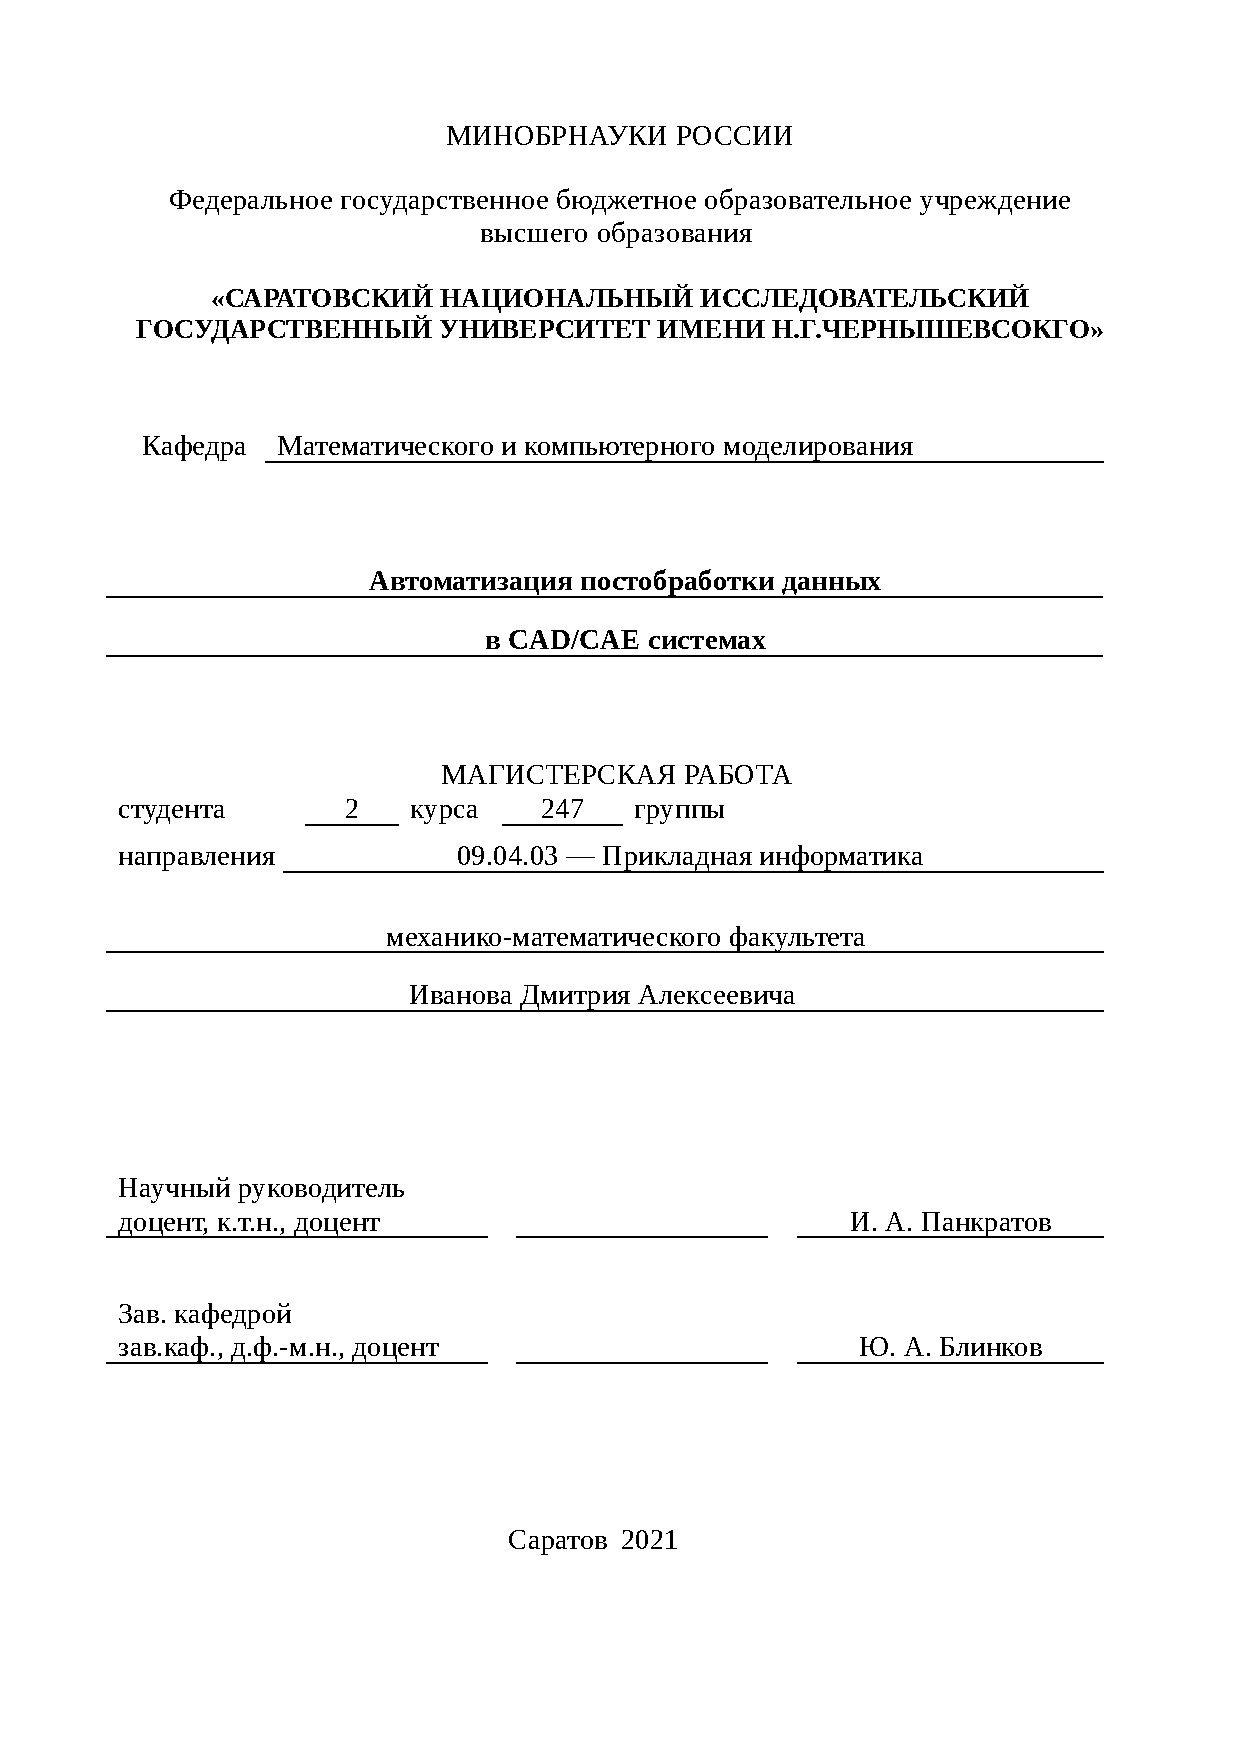
\includepdf[pages={1}]{titulCourse.pdf}

\tableofcontents

\intro
Введение должно включать:
\begin{itemize}
\item общую информацию о состоянии разработок по выбранной теме;  
\item обоснование актуальности и новизны темы, связь данной работы с другими научно-исследовательскими работами; 
\item цель работы и решаемые задачи. 
\end{itemize}

\chapter{Краткая информация об OpenFOAM и ParaView}
\section{OpenFOAM}
OpenFOAM (англ. Open Source Field Operation And Manipulation CFD ToolBox) — открытая интегрируемая платформа для численного моделирования задач механики сплошных сред. ~\cite{OpenfoamWiki}

Это пакет программ распространяемых свободно под лицензией GNU GPL, позволяющей решать задачи механики спошных сред, в частности: 
\begin{itemize}
\item Прочностные расчеты;
\item Гидродинамика ньютоновских и неньютоновских вязких жидкостей как в несжимаемом, \item так и сжимаемом приближении с учётом конвективного теплообмена и действием сил гравитации. Для моделирования турбулентных течений возможно использование RANS-моделей, LES- и DNS-методов. Возможно решение дозвуковых, околозвуковых и сверхзвуковых задач;
Задачи теплопроводности в твёрдом теле;
\item Многофазные задачи, в том числе с описанием химических реакций компонент потока;
\item Задачи, связанные с деформацией расчётной сетки;
\item Сопряжённые задачи;
\item Некоторые другие задачи, при математической постановке которых требуется решение дифференциальных уравнений в частных производных в условиях сложной геометрии среды;
\end{itemize}

В основе кода лежит набор библиотек, предоставляющих инструменты для решения систем дифференциальных уравнений в частных производных как в пространстве, так и во времени. Рабочим языком кода является C++. OpenFOAM состоит из приблизительно 250 программ основанных на более чем 100 библиотеках. Каждое приложения выполняет свою конкретную задачу в рамках процесса расчета. Этапы работы представленные в соответствии с рисунком ~\ref{fig}.

\begin{figure}[H]
\centerline{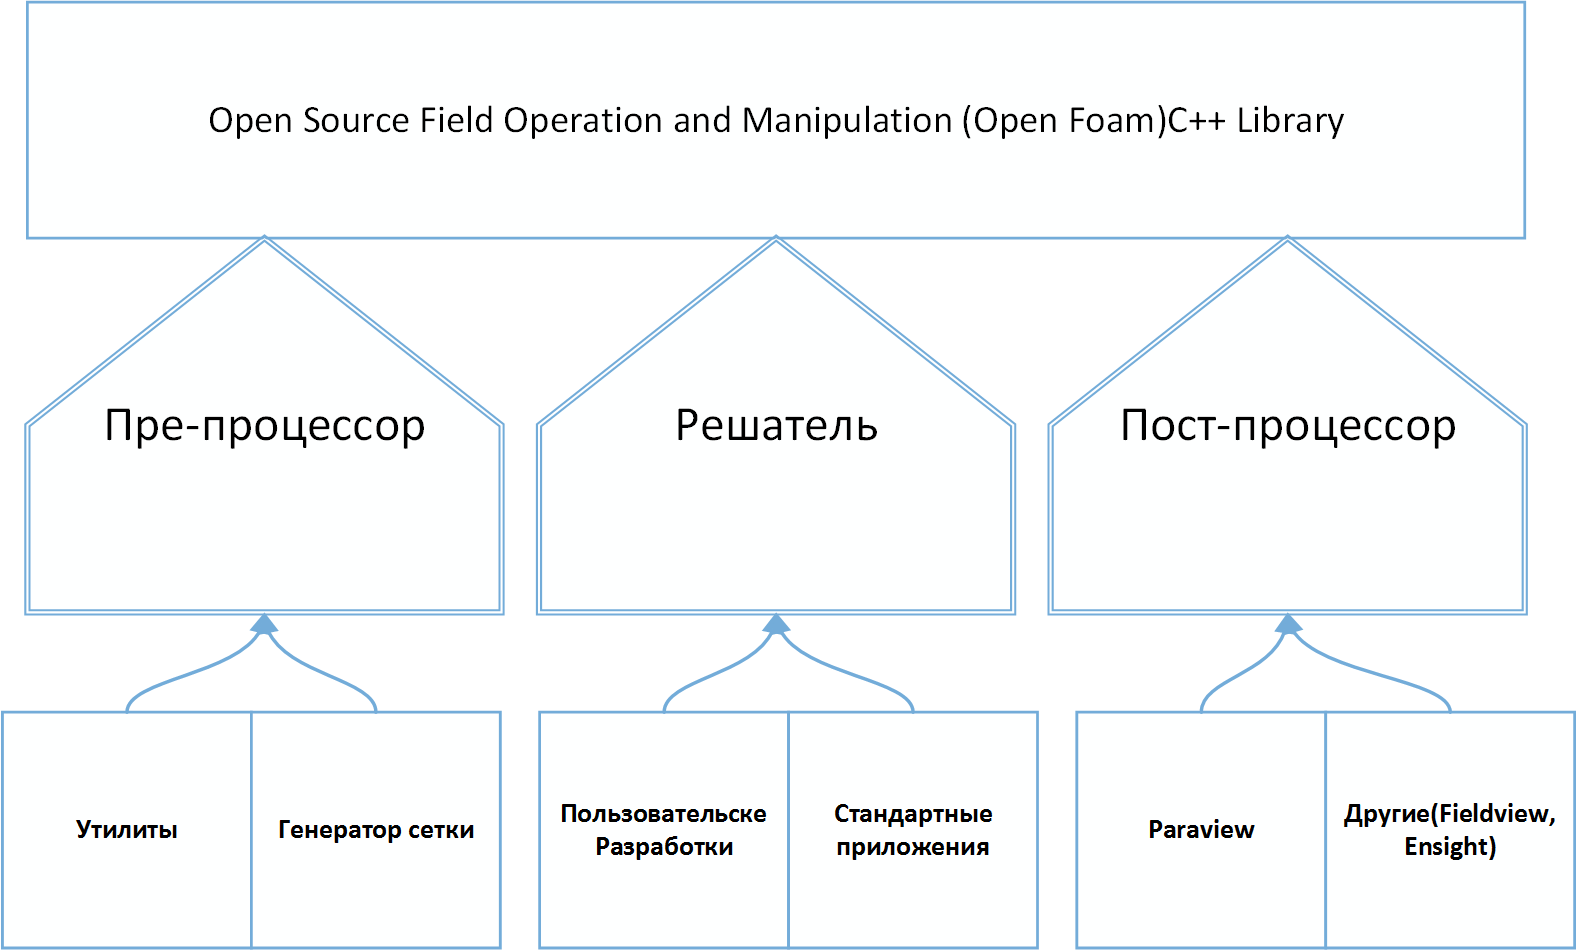
\includegraphics[width=1.0\linewidth]{OFScheme}}
\caption{Утилиты и программы входящие в пакет OpenFOAM, сгруппирвоанные по этапам работы с расчетом.}
\label{fig1}
\end{figure}

Работа с программой делится на три этапа:
\begin{enumerate}
\item Пре-процессинг;
\item Решение;
\item Пост-процессинг.
\end{enumerate}

На этапе пре-процессинга в специальных файлах задаются входные данные для рассчета примера, такие как: начальное время, конечное время, шаг и так далее. Также параметры для хранения решения: время, формат, тип сжатия. Также в препроцессинг включены настройки выбора различных схем рассчета, котоыре влияют на точность и стабильность решения. После этого отдельно генерируется расчетная область (сетка), которая вполседствии может быть обработана различными утилитами ~\cite{OpenfoamUserGuide}. Затем запускается решатель, который производит рассчет. На этапе пост-процессинга послученные данные представляются в виде графиков. Также используются некоторые утилиты, например для конвертации из внутреннего формата OpenFOAM в широко используемый формат vtk.

\section{ParaView}
ParaView -- открытый графический кросс-платформенный пакет для интерактивной визуализации в исследовательских целях, разрабатываемый Национальной Лабораторией Сандиа, компанией Kitware и Национальной Лабораторией Лос-Аламоса \cite{ParaviewAbout}.

Пакет ParaView предоставляет пользователю возможности интерактивной визуализации и исследования больших массивов данных для качественного и количественного анализа.

Пакет может быть использован на компьютерах с операционными системами Windows, Linux, Mac OS X.

При разработке авторы придерживаются следующих целей:
\begin{itemize}
\item Открытость, кросс-платформенность — в пакете используются только открытые, мульти-платформенные технологии для визуализации данных.
\item Поддержка различных, в том числе, гетерогенных вычислительных систем.
\item Создание гибкого, интуитивного пользовательского интерфейса.
\end{itemize}

Таким образом, пакет ParaView во многом является скорее технологией обработки, чем всего лишь программным средством ~\cite{ParaviewWiki}.

Одни из основных возможностей пакета:
\begin{itemize}
\item Визуализация расчетных областей.
\item Визуализация полей (давление, скорость, температура, смещения и прочее).
\item Построение срезов областей как плоскостью, так и заданной функцией.
\item Построение изо-поверхностей.
\item Построение векторных полей и линий тока.
\item Позволяет показывать динамику развития протекающего процесса, отображая анимацию. 
\end{itemize}

Основной формат данных ParaView -- VTK, но пакет также содержит драйверы для работы с форматом OpenFOAM и поставляется вместе с дистрибутивом пакета. 

Работа с Paraview может осуществляться как в интерактивном, так и пакетном режиме.
Приложение 

ParaView также предлагает богатый и мощный програмный интерфейс на языке Python. Это позволяет пользователям автоматизировать обработку своих данных и использовать возможности, так называемого, набора инструментов визуализации -- Visualization Tool Kit (VTK) ~\cite{ParaviewAndPython}. 




\conclusions

% Оформляем библиографию в соответствии с ГОСТ 7.0.5
\bibliographystyle{ugost2008}
% если хотим включить все источники из библиографии даже не имеющие ссылки из текта
% \nocite{*}
% файл с библиографией
\bibliography{biblio.bib}

% \Appendix % Приложения

\end{document}
